\documentclass{standalone}
\usepackage{tikz}
\usepackage{ctex,siunitx}
\setCJKmainfont{Noto Serif CJK SC}
\usepackage{tkz-euclide}
\usepackage{amsmath}
\usetikzlibrary{patterns, calc,3d}
\usetikzlibrary {decorations.pathmorphing,decorations.pathreplacing,decorations.shapes}
\begin{document}
\small
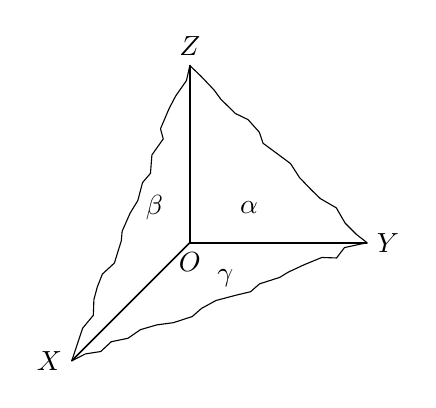
\begin{tikzpicture}[>=latex,scale=1.5]
  \tkzDefPoints{0/0/O,1.5/0/Y,0/1.5/Z,-1/-1/X}
  \tkzDrawSegments[semithick](O,X O,Y O,Z)
  \draw[decorate,decoration={random steps,segment length=2mm,amplitude=0.5mm}](X)--(Y);
  \draw[decorate,decoration={random steps,segment length=2mm,amplitude=0.5mm}](X)--(Z);
  \draw[decorate,decoration={random steps,segment length=2mm,amplitude=0.5mm}](Z)--(Y);
  \node at (-0.3,0.3){$\beta$};
  \node at (0.5,0.3){$\alpha$};
  \node at (0.3,-0.3){$\gamma$};
  \tkzLabelPoints[above](Z)
  \tkzLabelPoints(O)
  \tkzLabelPoints[right](Y)
  \tkzLabelPoints[left](X)
\end{tikzpicture}
\end{document}